%----------------------------------------------------------------------------------------
%	PACKAGES AND OTHER DOCUMENT CONFIGURATIONS
%----------------------------------------------------------------------------------------

\documentclass{article} % Paper and 12pt font size
\usepackage[utf8]{inputenc}
\usepackage{lmodern} % Use font Latin Modern Sans Typewriter
\usepackage[a4paper, margin=1in]{geometry} % Paper size and margin

\usepackage{enumitem} % Format the enumerated list
\usepackage{amsmath,amsfonts,amsthm,mathtools,commath,bm} % Math packages
\setlength\parindent{0pt} % Removes all indentation from paragraphs - comment this line for an assignment with lots of text

\usepackage{array}
\usepackage{tabu} % Table to text width
\renewcommand{\arraystretch}{0.6} % If the value is 1.0, the height of each row in the table is set to 1.5 relative to its default height. Adjust based on that.
\usepackage[table]{xcolor}

\usepackage{tikz} % Remember picture
\usepackage{graphicx} % Includes images
\graphicspath{ {./images/} } % Tells LATEX that the images are kept in a folder named images under the directory of the main document
\usepackage{subcaption}
\usepackage{wrapfig} % Wrap image i
\usepackage{eso-pic} % used for image background on titlepage

% Code listing style --------------
\usepackage{listings} % Code listing
\usepackage{color}
\definecolor{codegreen}{rgb}{0,0.6,0}
\definecolor{codegray}{rgb}{0.5,0.5,0.5}
\definecolor{codepurple}{rgb}{0.58,0,0.82}
\definecolor{backcolour}{rgb}{0.95,0.95,0.92}
\lstdefinestyle{mystyle}{
    backgroundcolor=\color{backcolour},
    commentstyle=\color{codegreen},
    basicstyle=\ttfamily\small,
    keywordstyle=\color{magenta},
    numberstyle=\tiny\color{codegray},
    stringstyle=\color{codepurple},
    breakatwhitespace=false,
    breaklines=true,
    captionpos=b,
    keepspaces=true,
    numbers=left,
    numbersep=5pt,
    showspaces=false,
    showstringspaces=false,
    showtabs=false,
    tabsize=2
}
\lstset{style=mystyle}

%----------------------------------------------------------------------------------------
%	TITLE SECTION
%----------------------------------------------------------------------------------------
\title{\Huge \textbf{Report on Generalized Linear Model with Basis Functions and Kernels} \vspace{.4in} \hrule}

\author{%\LARGE University of Toronto Institute for Aerospace Studies\\
  \vspace{0.5cm}
	\Large ROB313: Introduction to Learning from Data \\
  \vspace{0.5cm}
	\Large Yizhi (Jojo) Zhou, 1003002396\\
}
\date{\normalsize\today}

\linespread{1.5}

\begin{document}
	\begin{titlepage}
	\tikz[remember picture,overlay]
	\node[yshift=8.0cm] at (current page.south){
\includegraphics[width=\paperwidth]{404.png}};%height=\paperheight and (current page.south)
	\vspace*{3.5cm}
  {\let\newpage\relax\maketitle}
	\vspace*{\fill}

	\end{titlepage}

\newpage

%----------------------------------------------------------------------------------------
%	PROBLEM 1
%----------------------------------------------------------------------------------------
\vspace{0.4cm}
\section*{Objectives} % The * makes it an unnumbered section
The Generalized Linear Model(GLM) predicts a value by finding the mathetatical relationship between the features and labels in the dataset. Like linear regression, GLM finds weight parameters to minimize the loss, but unlike linear regression, the weights correspond to $\phi(x)$, which maps x to a different space so that the linear model can be used on nonlinear datasets.

The following report discusses the GLM basis function and kernel used for the mauna\_loa dataset, and then the Radial Basis Function(RBF)'s performance on three different datasets.


%----------------------------------------------------------------------------------------
%	PROBLEM 1
%----------------------------------------------------------------------------------------
\vspace{0.4cm}
\section*{Solution Structure and Strategies} % The * makes it an unnumbered section
The GLM implementation consists of three classes:
\begin{itemize}
  \item \textbf{GLM.} This class is initiated with the name of dataset of interest, which is loaded and preprocessed for the convenience of prediction. The prediction function initiates a \textbf{BasisFunctions} or \textbf{Kernels} object, which takes in the hyperparameters (e.g. degree, $\theta$) along with the training set to find the parameters (\textbf{w}, \textbf{$\alpha$}) and basis functions $\Phi(x)$ or the Gram Matrix. It then computes the prediction as a product of them. Finally, it visualizes the prediction and shows the Root-Mean-Square-Error(RMSE) for the regression datasets, and the accuracy for the classification datasets.

  \item \textbf{BasisFunctions.} This class has three main functions, one being the parameter calculation function that uses Singular Value Decomposition(SVD) to compute the weights for loss minimization using \textbf{$w = V(\Sigma+\lambda I)^{-1}\Sigma^TU^Ty$}, one being a high-level function to translate the specified dataset into matrix \textbf{$\Phi(x)$}, and the last one being the basis function that takes a single data point $x^{(i)}$ and maps it to vector $\{\phi_0(x^{(i)}) ... \phi_{M-1}(x^{(i)})\}^T$. Multiple basis functions are implemented, including Polynomial and Gaussian. The final model is specifically tailored for mauna\_loa, which will be demonstrated in the next section.

  \item \textbf{Kernels.} Sharing the same structure as the \textbf{BasisFunctions} class, the \textbf{Kernels} class differs by using computing the Gram Matrix K instead of the \textbf{$\Phi(x)$} matrix, and that it finds the $\alpha = (K+\lambda I)^{-1}y)y$ parameter instead of weights, through Cholesky Factorization. Likewise, multiple different Kernels are implemented including Polynomial, Gaussian, and the kernel trick that is directly transferred from the basis function for mauna\_loa.

\end{itemize}



%----------------------------------------------------------------------------------------
%	PROBLEM 2
%----------------------------------------------------------------------------------------
\vspace{0.4cm}
\section*{Basis Function on Dataset Mauna\_loa} % The * makes it an unnumbered section

\textbf{Basis function design}

  The mauna\_loa dataset is one-dimensional. Through visualization, it is obvious that there is a general incresasing trend of $y$ almost directly proportional to $x$, along with seasonal sinusoidal patterns which has the same period. Therefore, the basis function maps $x$ to a polynomial and a sinusoidal model. The degree of polynomial is determined by experimentation of different degrees with cross-validation, which leads to a $4^{th}$ order polynomial. The period of sinusoidal model is calculated by $2\pi / T$, with the period $T$ observed to be 0.057.

\textbf{Regularization factor selection}

  To choose a suitable regularization factor, the training and validation sets are combined to predict the test set, using the basis function described above. The results are shown in the left half of Table 1, along with a visualization with the chosen $\lambda = 0$ in the left picture of Figure 1.

  % Table for cross-validation
  \begin{table}[!ht]
  \begin{minipage}{0.51\textwidth}
  \raggedleft
  \scalebox{1.4}{\begin{tabular}[t]{||r | c c||}
      \hline
      \rowcolor{lightgray}\multicolumn{3}{||c||}{RMSE with Basis Functions}\\
      $\lambda$  & Validation & Test Set \\
      \hline
      \cellcolor{yellow}0 &    \cellcolor{yellow}0.055632 &  \cellcolor{yellow}0.044172 \\
      0.0001 &    0.055645 &  0.044174 \\
      0.001 &    0.055764 &  0.044196 \\
      0.01 &    0.056951 &  0.044413 \\
      0.1 &    0.068950 &  0.046627 \\
      1 &    0.178556 &  0.071051 \\
      \hline
      % \rowcolor{pink}\multicolumn{3}{||c||}{Test Set RMSE: 0.249432}\\
      % \hline
  \end{tabular}}
  \end{minipage}
  \hspace{0.01\textwidth}
  \begin{minipage}{0.51\textwidth}
  \raggedright
  \scalebox{1.4}{\begin{tabular}[t]{||r | c c||}
      \hline
      \rowcolor{lightgray}\multicolumn{3}{||c||}{RMSE with the Kernel Method}\\
      $\lambda$  & Validation & Test Set \\
      \hline
      1e-10 &    0.055682 &  0.044191 \\
      1e-08 &    0.055633 &  \cellcolor{yellow}0.044172 \\
      \cellcolor{yellow}1e-06 &    \cellcolor{yellow}0.055632 &  \cellcolor{yellow}0.044172 \\
      0.0001 &    0.055636 &  \cellcolor{yellow}0.044172 \\
      0.01 &    0.056005 &  0.044230 \\
      1 &    0.092373 &  0.050248 \\
      \hline
      % \rowcolor{pink}\multicolumn{3}{||c||}{Test Set RMSE: 0.249432}\\
      % \hline
      \end{tabular}}
  \end{minipage}
  \caption{RMSE results of the mauna\_loa dataset}
  \end{table}

  \begin{figure}[!ht]
    \centering
    \begin{subfigure}[b]{0.48\linewidth}
      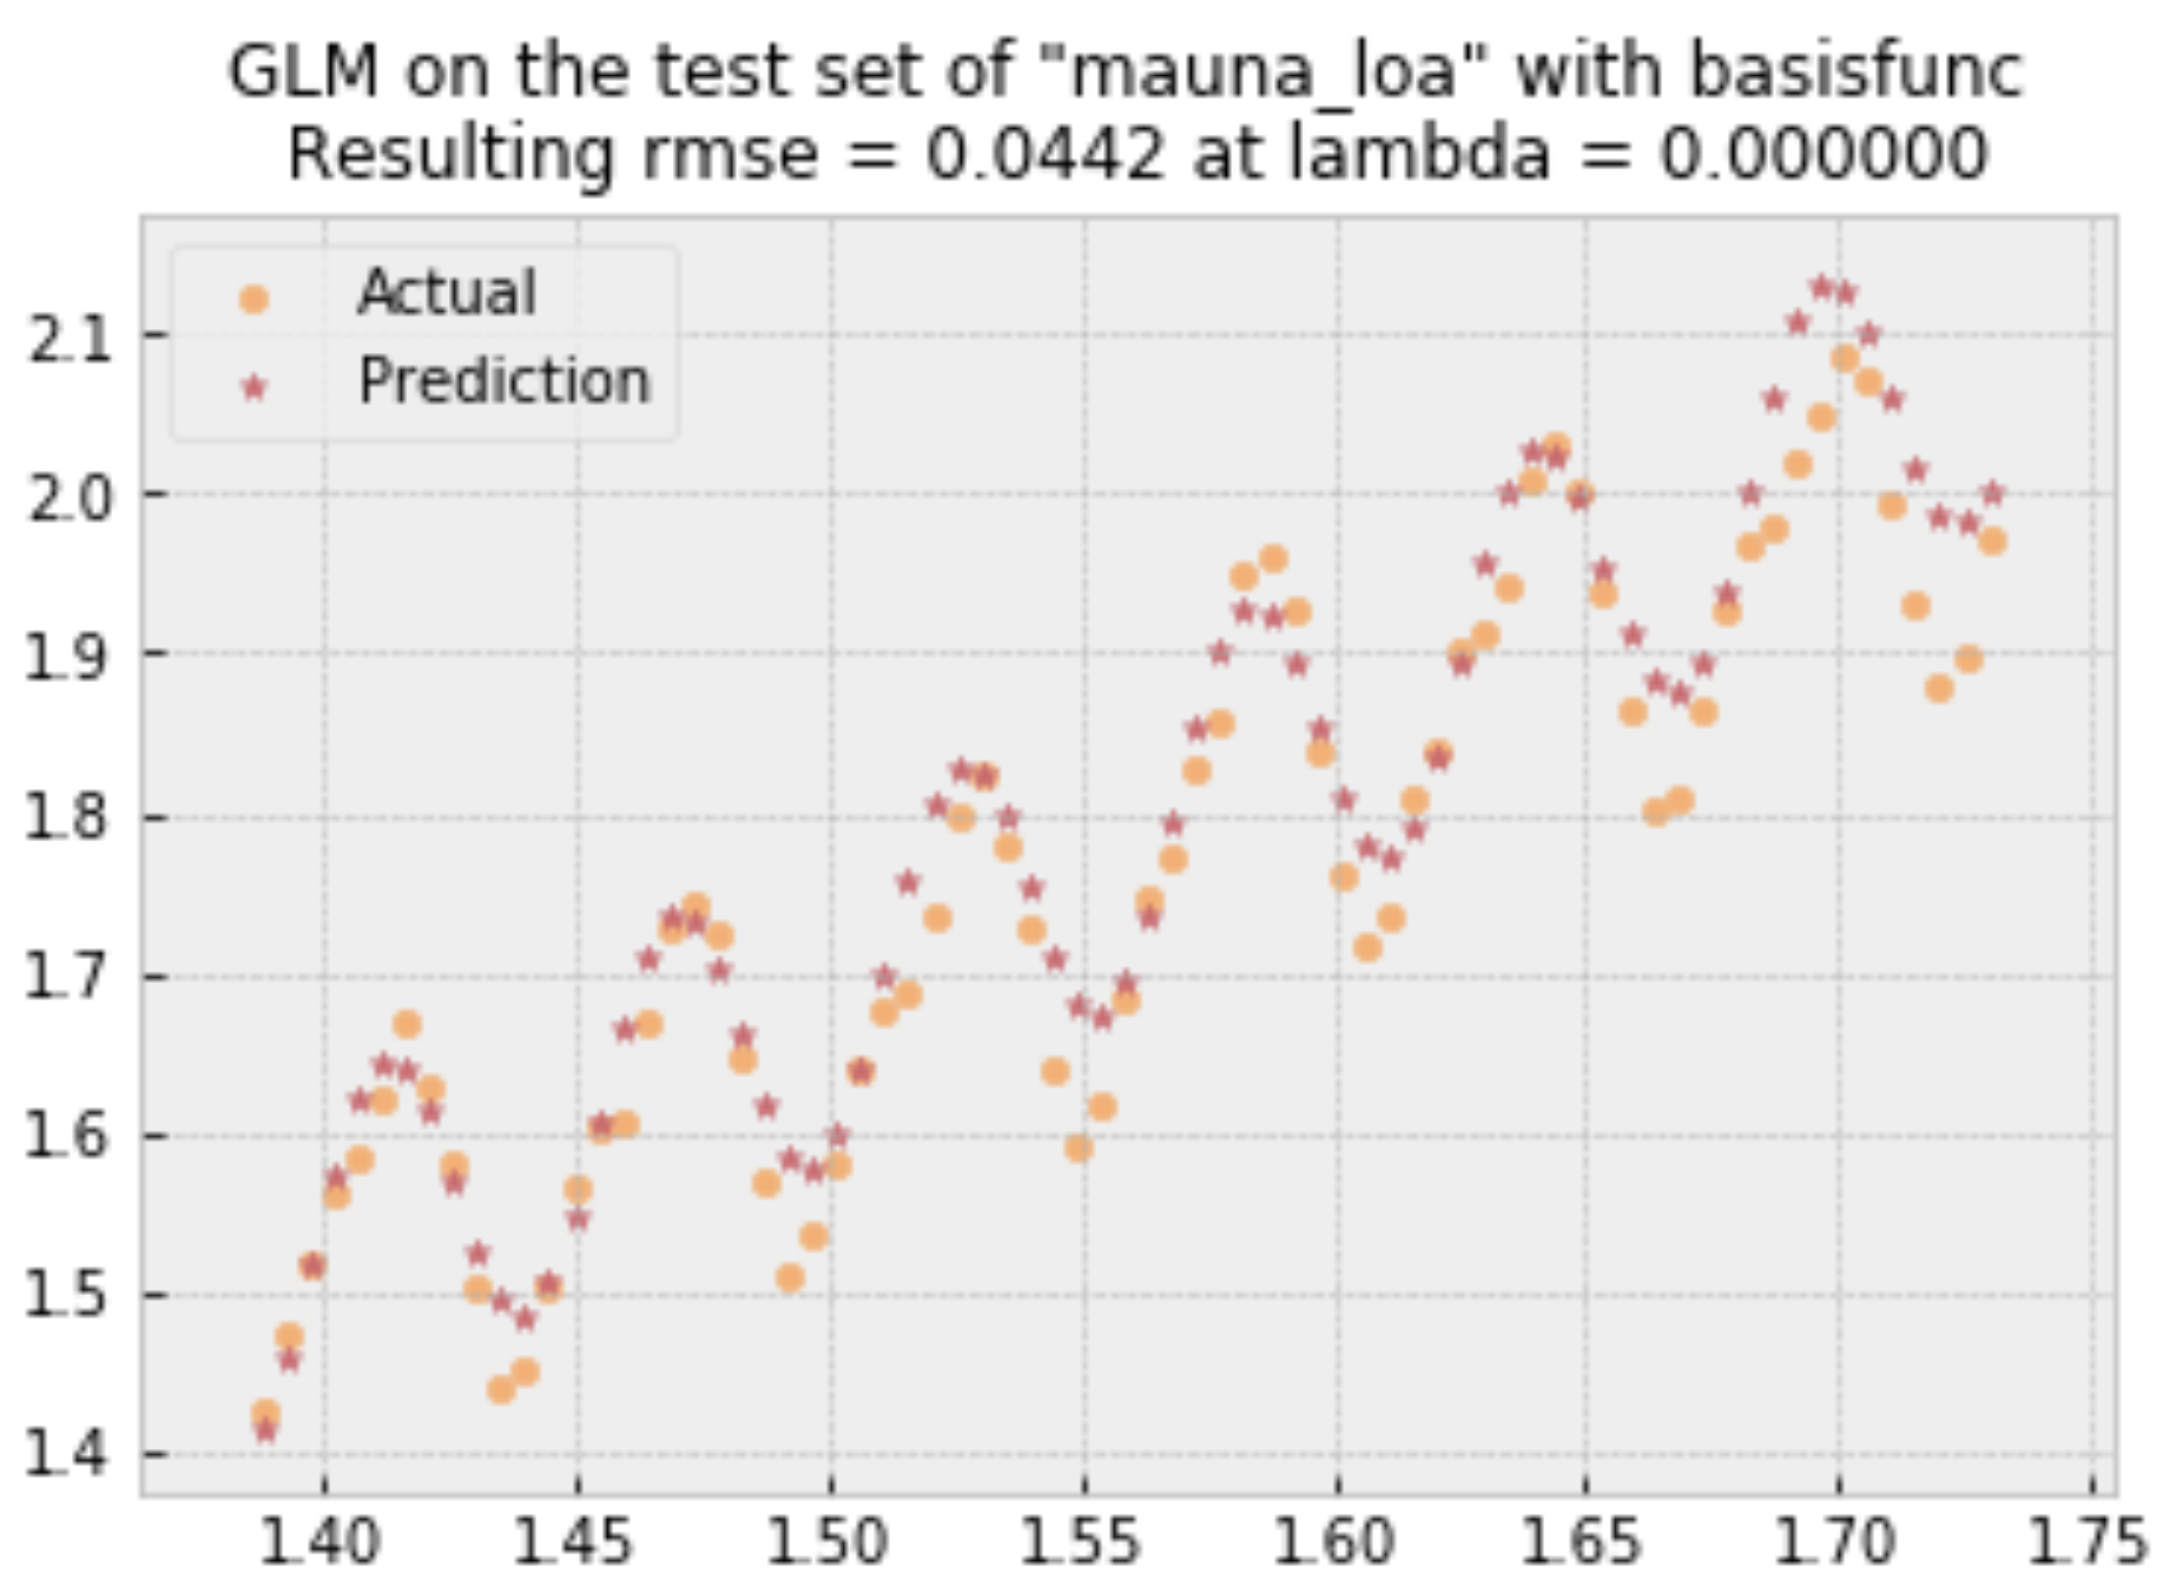
\includegraphics[width=\linewidth]{Q1.png}
      \caption{Prediction with basis function on dataset mauna\_loa}
    \end{subfigure}
    \begin{subfigure}[b]{0.48\linewidth}
      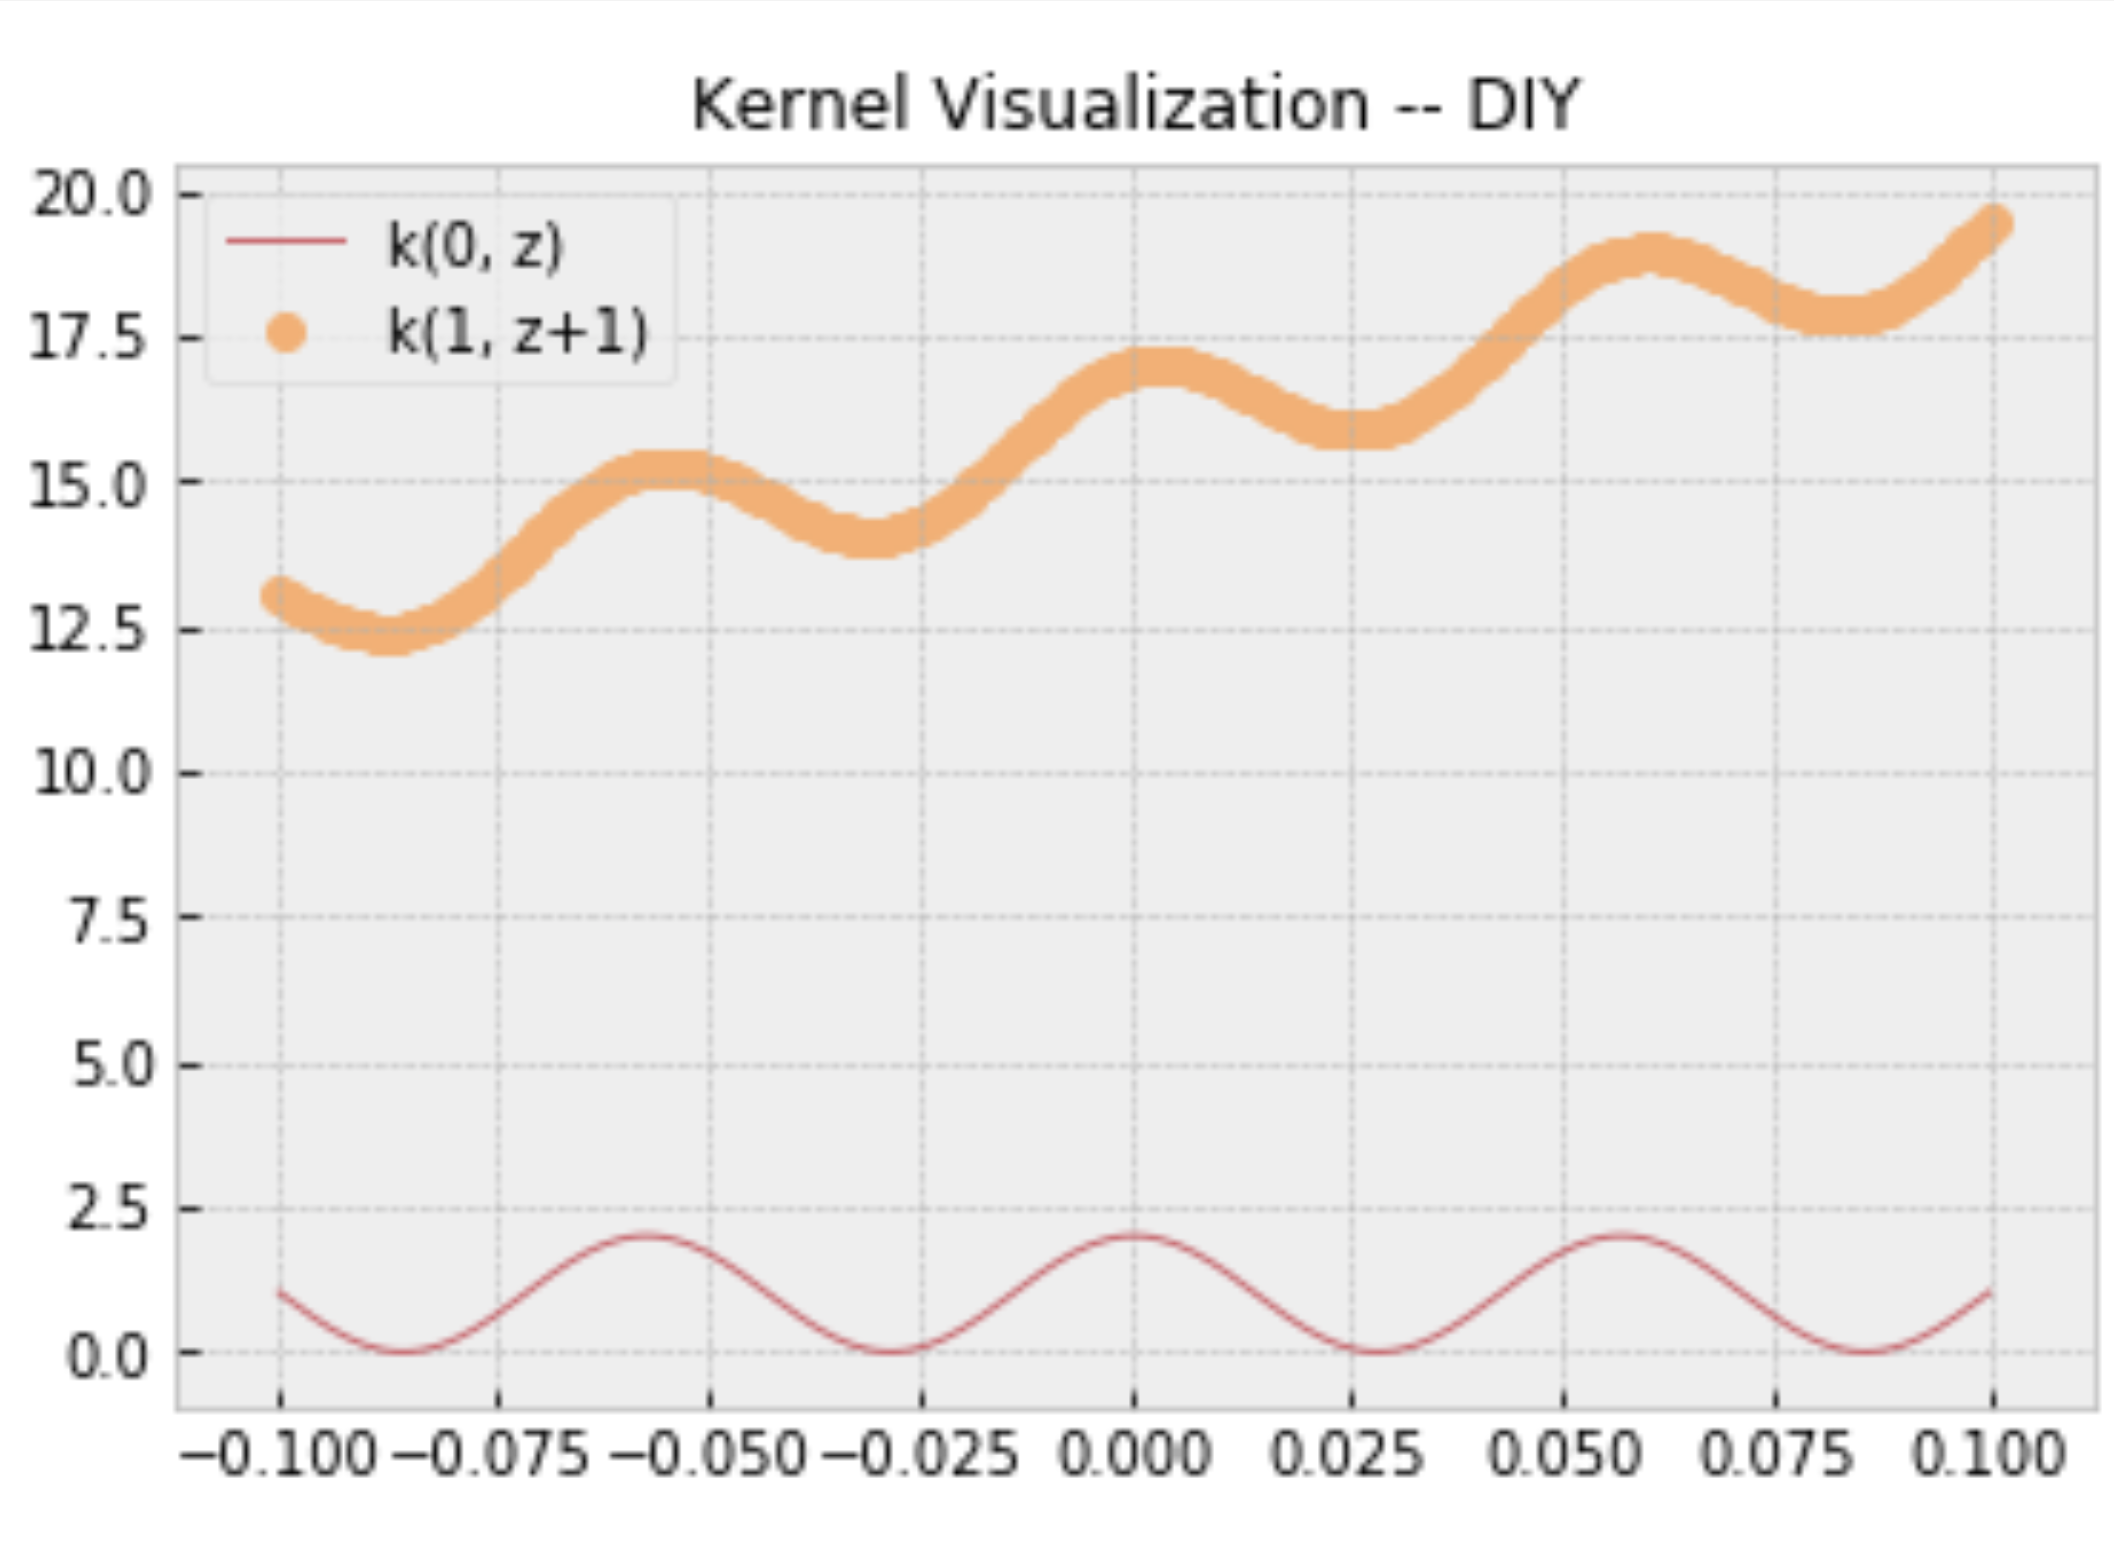
\includegraphics[width=\linewidth]{Q2.png}
      \caption{Visualization of the kernel based on the same basis function}
    \end{subfigure}
    \caption{Visualizations for Question 1 and 2}
    \label{fig:Q12}
  \end{figure}


\vspace{0.2cm}
%----------------------------------------------------------------------------------------
%	PROBLEM 1
%----------------------------------------------------------------------------------------
\vspace{0.4cm}
\section*{Kernel Method on Dataset Mauna\_loa} % The * makes it an unnumbered section

\textbf{Kernel design}

The kernel $k(x, z) = \phi(x)^T \phi(z)$ is based on the basis function $\phi$ used in the previous part. This dot product is equivalent to $k = 1 + xz + x^2z^2 + ... + x^dz^d + sin(2\pi x/T)sin(2\pi z/T) + cos(2\pi x/T)cos(2\pi z/T) = (1+x^Tz)^d + cos(2\pi(x-z)/T)$ with the same parameters degree d = 4 and period T = 0.057.

The kernel is visualized in the right picture of Figure 1. It is clear that $k(x, z)$ changes when $x, z$ are increased by the same amount. Since the kernal is not dependent on only the distance between two inputs (i.e. $k(x, z)\neq k(x-z)$), it is not translational invariant or stationary.

\textbf{Regularization factor selection}

Same as the previous question, the RMSEs corresponding to different regularization factors are shown on the right of Table 1. In the case of kernel method, $\lambda$ cannot be 0, otherwise $(K + \lambda I)$ is not positive definite and cannot be factorized by the Cholesky method. Here, the minimum is occurs roughly when $\lambda$ is close to 0.

\textbf{Primal approach vs. dual approach}

The primal appraches computes the N-by-M $\Phi(x)$ while dual approach computes the N-by-N Gram matrix. In this case where $M<<N$, the gram matrix is significantly larger than $\Phi(x)$. Meanwhile, these matrices are needed in the compulation of weight and $\alpha$, which further aggravates the impact of a large Gram matrix and dominates the runtime. With SVD on $\Phi(x)$, it takes $O(NM^3)$ time to compute the weights, and the Gram matrix takes $O(N^3)$ with Cholesky to compute $\alpha$. Therefore, the dual approach's time complexity is worse than the primal approach, on the mauna\_loa dataset. Likewise, the memories required to store the matrix is also smaller for the primal approach $O(NM)$ than dual approach ($O(N^2)$).


%----------------------------------------------------------------------------------------
%	PROBLEM 3
%----------------------------------------------------------------------------------------
\vspace{0.4cm}

\section*{Gaussian RBF Kernel on Various Datasets} % The * makes it an unnumbered section

\begin{table}[!hb]
\centering
\scalebox{1.1}{\begin{tabular}[t]{|r | c c c c c|}
  \hline
  \hline
  $\lambda$  &      \cellcolor{yellow}$\theta=0.05$ &       $\theta=0.1$ &       $\theta=0.5$ &         \cellcolor{pink}$\theta=1$ &         \cellcolor{cyan}$\theta=2$ \\
  \hline
  \rowcolor{lightgray}\multicolumn{6}{|c|}{RMSE on dataset "mauna\_loa"}\\
  \hline
  \cellcolor{pink}0.001 &  1.219709 &  1.416286 &  0.347101 &  \cellcolor{pink}0.124479 &  0.201705 \\
  0.01 &  1.117309 &  1.059137 &  0.427720 &  0.229495 &  0.252404 \\
  0.1 &  1.082018 &  0.965908 &  0.473741 &  0.339112 &  0.217145 \\
  1 &  1.092211 &  0.996726 &  0.606334 &  0.443615 &  0.249220 \\
  \hline
  \rowcolor{lightgray}\multicolumn{6}{|c|}{RMSE on dataset "rosenbrock"}\\
  \hline
  \cellcolor{cyan}0.001 &  0.735463 &  0.626585 &  0.351507 &  0.257236 &  \cellcolor{cyan}0.193240 \\
  0.01 &  0.738913 &  0.632028 &  0.381007 &  0.297407 &  0.241027 \\
  0.1 &  0.752307 &  0.647735 &  0.419093 &  0.358185 &  0.311707 \\
  1 &  0.808103 &  0.720521 &  0.513313 &  0.466635 &  0.436547 \\
  \hline
  \rowcolor{lightgray}\multicolumn{6}{|c|}{Accuracy on dataset "iris"}\\
  \hline
  0.001 &  \cellcolor{yellow}0.806452 &  0.838710 &  0.838710 &  0.838710 &  0.838710 \\
  \cellcolor{yellow}0.01 &  \cellcolor{yellow}0.806452 &  0.838710 &  0.838710 &  0.838710 &  \cellcolor{yellow}0.806452 \\
  \cellcolor{yellow}0.1 &  \cellcolor{yellow}0.806452 &  \cellcolor{yellow}0.806452 &  0.838710 &  0.838710 &  0.838710 \\
  1 &  \cellcolor{yellow}0.806452 &  \cellcolor{yellow}0.806452 &  0.870968 &  0.870968 &  0.870968 \\
  \hline
  \hline
\end{tabular}}
\caption{Performance of Gaussian RBF Kernel on each dataset with different $\lambda$ and $\theta$ values}
\end{table}

\begin{figure}[!hb]
  \centering
  \begin{subfigure}[b]{0.48\linewidth}
    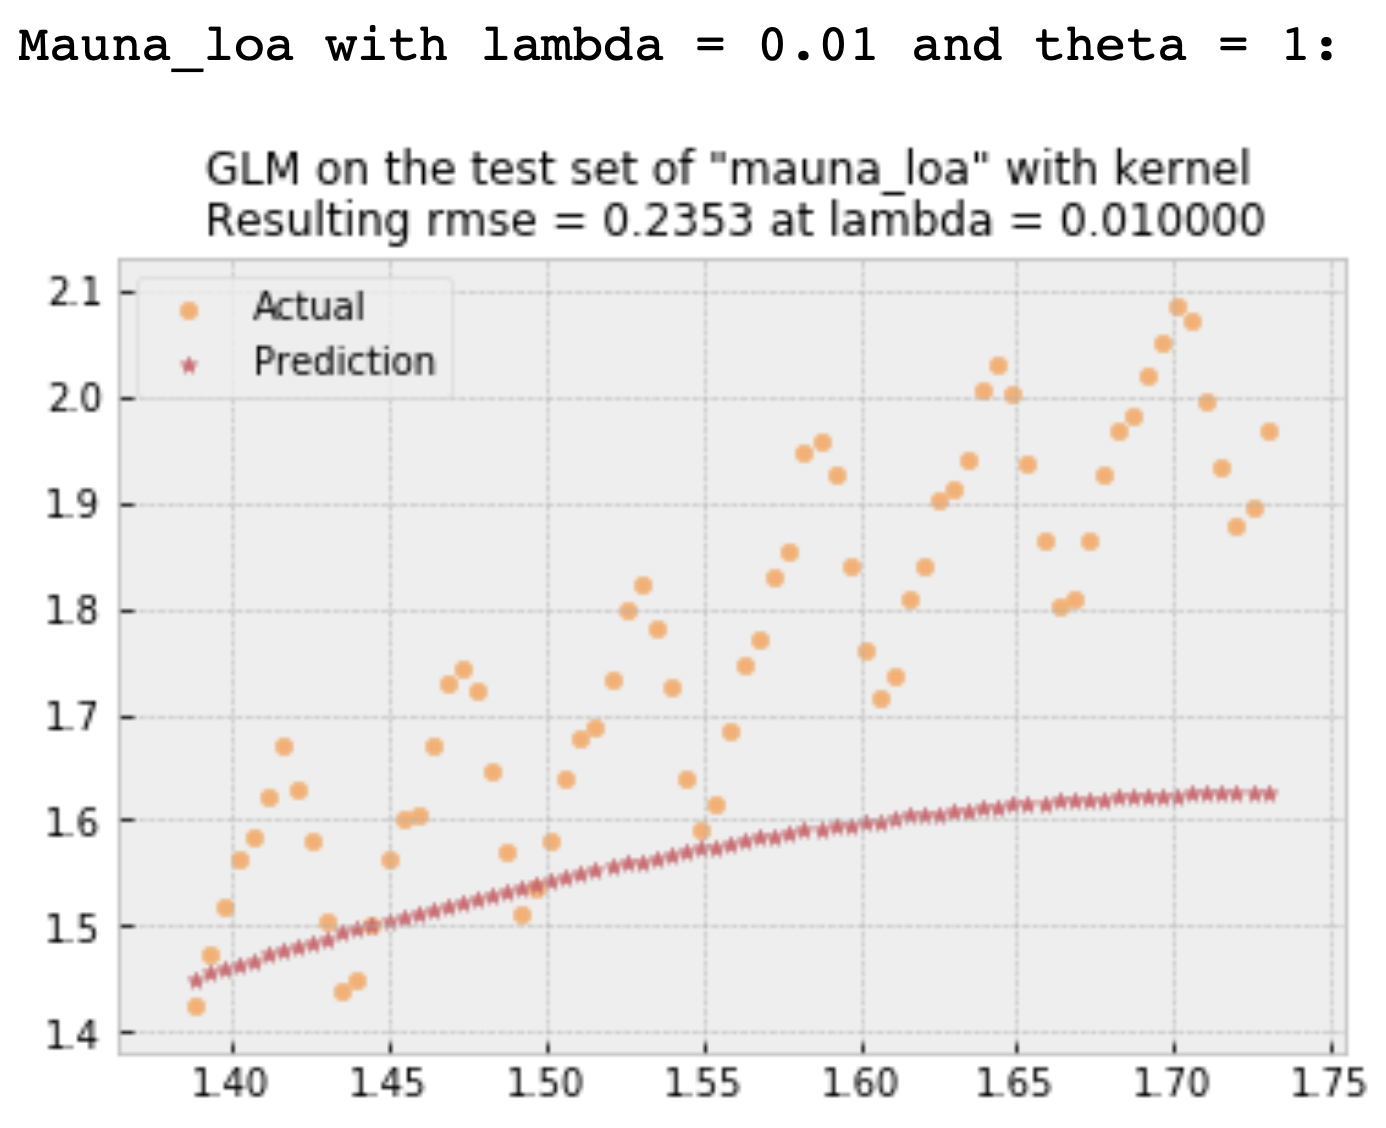
\includegraphics[width=\linewidth]{Q3_1.png}
    \caption{Dataset mauna\_loa}
  \end{subfigure}
  \begin{subfigure}[b]{0.48\linewidth}
    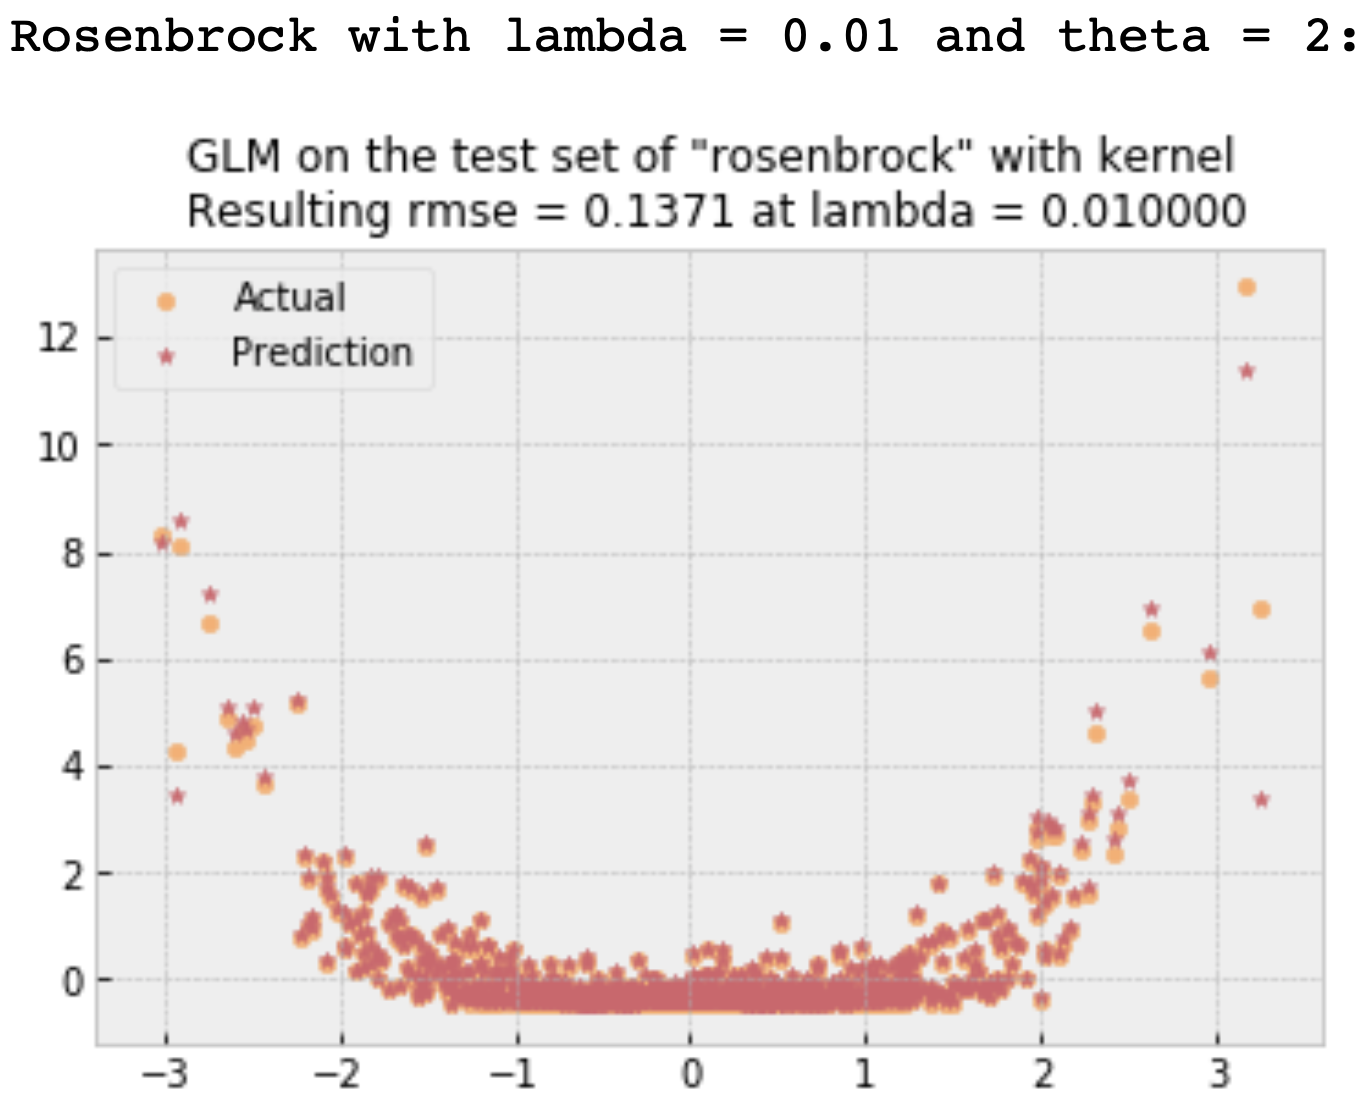
\includegraphics[width=\linewidth]{Q3_2.png}
    \caption{Dataset rosenbrock}
  \end{subfigure}
  \caption{Visualizations for the test results with the optimal conditions from above}
  \label{fig:Q3}
\end{figure}

The Gaussian RBF kernel is implemented by commupting $k(x,z) = exp(\frac{||x-z||_2^2}{\theta})$ and Cholesky factorization. The grid of lengthscales $\theta = \{0.05, 0.1, 0.5, 1, 2\}$ and the grid of regularization parameters $\{0.001, 0.01, 0.1, 1\}$ are tested on datasets mauna\_loa, rosenbrock, and iris. The results and optimal parameters on the validation set for each dataset are marked in pink, blue, and yellow, respectively. The prediction performance on the test sets are then shown in Figure 2 below for the regression sets, and that of the classification dataset iris is 100\% accurate.



%----------------------------------------------------------------------------------------
%	PROBLEM 4
%----------------------------------------------------------------------------------------
\vspace{0.4cm}
\section*{Minimizer Derivation I}
\textbf{Problem}: Derive the minimizer of a linear regression model with a least-squares loss and general Tikhonov regularization whose training problem is defined as follows
$$argmin_{w\in \mathbb{R}^D} ||y - Xw||^2 + w^T\Gamma w$$
where $\Gamma\in \mathbb{R}^D$ is a symmetric positive semi-definite matrix.

\textbf{Solution}:
$$L(w) = (y-Xw)^T(y-Xw)+ w^T\Gamma w$$
$$\nabla_wL = -2X^T(y-Xw)+ 2\Gamma w = 0$$
$$(X^TX+\Gamma)w = X^Ty$$
$$w = (X^TX+\Gamma)^{-1}X^Ty$$


%----------------------------------------------------------------------------------------
%	PROBLEM 5
%----------------------------------------------------------------------------------------
\vspace{0.4cm}
\section*{Minimizer Derivation II}
\textbf{Problem}: Considering the GLM
$$\hat f(x, \alpha) = \Sigma_{i=1}^N \alpha_i k(x, x^{(i)})$$ derive a computational strategy to estimate $\alpha = \{\alpha_1, ... \alpha_N\}^T\in \mathbb{R}^N$ by minimizing the objective function $\Sigma_{i=1}^N (y^{(i)}-\hat f(x^{(i)}, \alpha))^2+ \lambda\Sigma_{i=1}^N \alpha_i^2$. Compare this expression for the weights to those we derived in class using the dual representation. Are they different or the same? Explain why.

\textbf{Solution}:

Let $\alpha = \begin{bmatrix} \alpha_1 \\.\\.\\.\\ \alpha_N \end{bmatrix} \in \mathbb{R}^N$,
$K = \begin{bmatrix} k(x^{(1)}, x^{(1)}) &...& k(x^{(N)}, x^{(1)}) \\ ...& . & . \\  . & . & ...\\ ...& . & . \\k(x^{(N)}, x^{(1)}) &...& k(x^{(N)}, x^{(N)}) \end{bmatrix}\in \mathbb{R}^{N \times N}$,
and
$\hat y = \begin{bmatrix} \hat f(x^{(1)}, \alpha)\\.\\.\\.\\ \hat f(x^{(N)}, \alpha) \end{bmatrix} \in \mathbb{R}^N$
Then $y = \{y^{(1)}, ... y^{(N)}\}^T$ and $\hat y = K\alpha$, the loss function can be rewriten as:
$$L(\alpha) = (y-K\alpha)^T(y-K\alpha)+ \alpha^T\lambda\alpha$$
$$\nabla_\alpha L = -2K^T(y-K\alpha)+ 2\lambda\alpha = 0$$
$$(K^TK+\lambda I)\alpha = K^Ty$$
$$\alpha = (K^TK+\lambda I)^{-1}K^Ty$$
Recall that the weights of dual representation is $w = (\Phi^T\Phi+\lambda I)^{-1}\Phi^Ty$ and $\alpha = (K + \lambda I)^{-1}y$, $\alpha$ here is different from $\alpha$ in the dual representation, but in the same form of the weights' expression with $\Phi$ replaced by K. This is because as the loss function used to get $\alpha$ is in the exact same form as that to get the weights, interchanging $\alpha$ and $w$, and K and $\Phi$. In the derivation of the $\alpha$ in dual representation, however, $w$ in the loss function is replaced by not $\alpha$ but $\Phi(x)^T\alpha$, which generates a  $\Phi(x)\Phi(x)^T$ in the regularization term, leading to the $\alpha$ used in the previous parts. That being said, $\alpha$'s actual value is still going to be different from both the $\alpha$ and $w$ in dual representation, as $\Phi$ is different from K in the end.







%----------------------------------------------------------------------------------------
%	Conclusion
%----------------------------------------------------------------------------------------
\vspace{0.4cm}
\section*{Conclusion} % The * makes it an unnumbered section
Through experimenting with different methods of GLM implementation, this project provides a practical understanding of when each basis function/kernel is suitable to use, and a chance to practice designing basis functions depending on a specific dataset. Meanwhile, through comparing the performance on different parameters, this project reinforces the intuitive of each parameter's effect on the prediction.
Last but not least, two computational strategies to minimize the loss function are derived and showed the impact on how a loss function is defined and the use of key parameters.
\end{document}
